\subsection{Transient creep in rock salt}
\label{subsec:Mc4}

\subsubsection{Definition}
\label{subsubsec:Mc4_def}

Triaxial long-term compression under axisymmetric conditions is carried out to verify the Lubby2 creep model Eq.~(\ref{Mc_lubby2_ec}), and to study transient as well as stationary creep behavior assuming isothermal conditions and neglecting damage processes.

\subsubsection{Solution}
\label{subsubsec:Mc4_sol}

As described in Sec.~\ref{subsec:Me6}, for the calculation, the cross-section of a cylindrical sample with a radius of $30\,$mm and a height of $120\,$mm is studied. The loading in principal axes includes a radial pressure as well as an axial pressure, and is realized in two steps. It is resulting in a homogeneous stress-strain state. Details of the model (geometry, mesh, boundary conditions) according to K.-H. Lux and F. Werunsky (unpublished report, 2008) are presented in Fig.~\ref{Mc_triax_model_lubby2}.

\begin{figure}[!htb]
\begin{center}
\includegraphics[width=0.2\textwidth]{PART_II/M/svv_model.eps}
\hspace*{10.0ex}
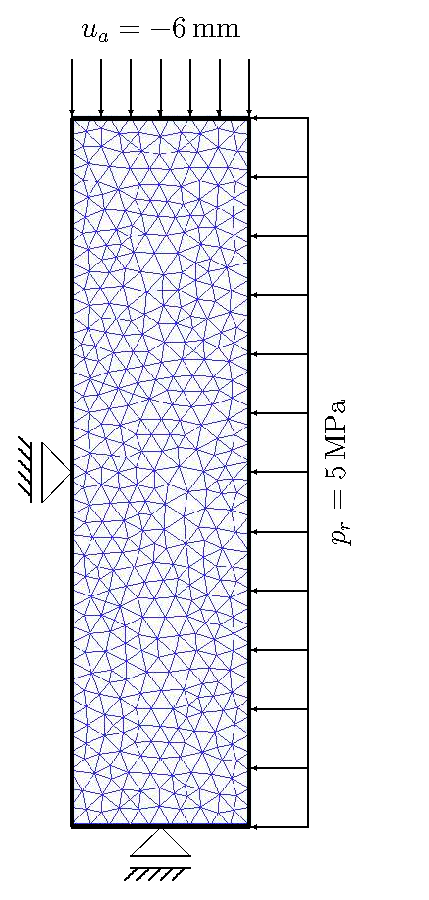
\includegraphics[width=0.25\textwidth]{PART_II/M/svv_mesh.eps}
\end{center}
\caption{Triaxial compression of a cylindrical sample. Axisymmetric model. Left: Geometry. Right: Finite element grid and boundary conditions.} 
\label{Mc_triax_model_lubby2}
\end{figure}

Initial conditions do not have to be given for the problem under consideration. As the bottom edge is fixed in vertical direction, the left-hand edge is fixed in horizontal direction for symmetry reasons (axis of rotation). On the right-hand edge initially a radial casing pressure of $5\,$MPa is applied within 60~seconds with a constant stress rate. While keeping constant this radial pressure, a subsequent stress-driven axial compressive loading is applied within the following 1440~seconds with a constant stress rate. The maximum axial pressure is $18\,$MPa. In the following, both the radial and the axial pressures are kept constant for 20~days (for the loading history cf. Fig.~\ref{Mc_triax_loadhist_lubby2}).

%\clearpage

\begin{figure}[!htb]
\begin{center}
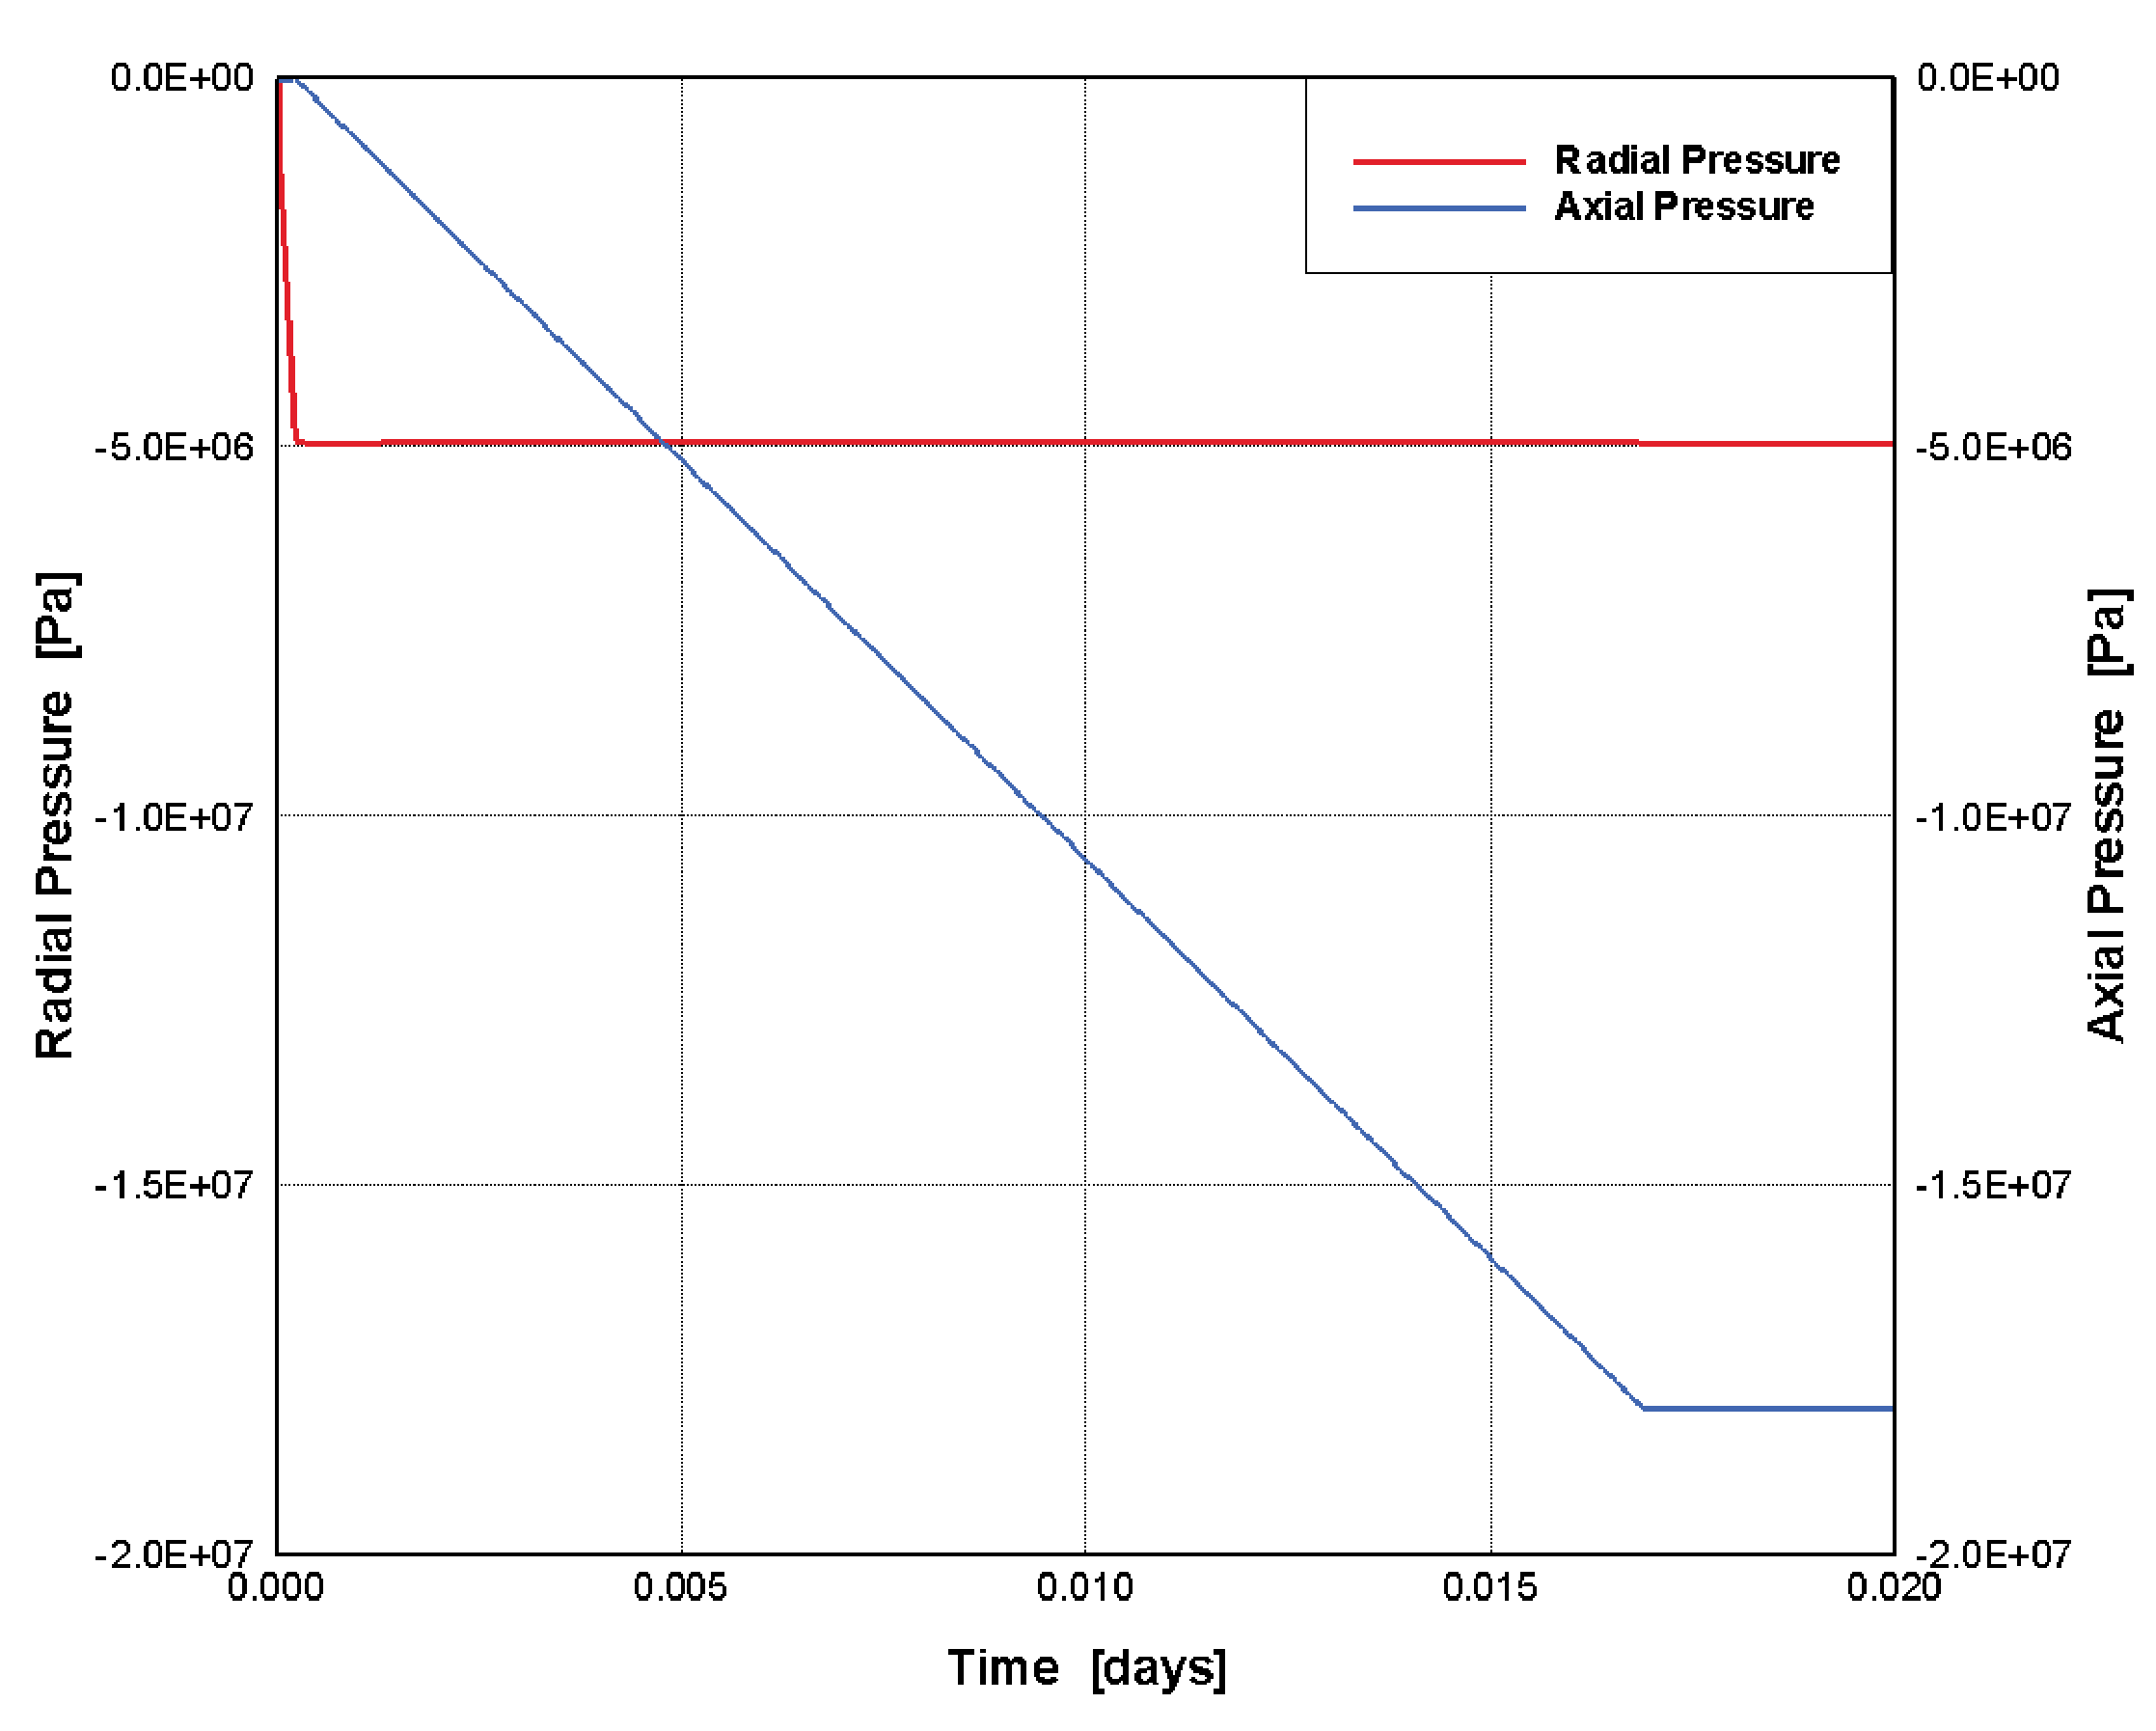
\includegraphics[width=0.6\textwidth]{PART_II/M/svvcreep_e_HL_loadhistory.eps}
\end{center}
\caption{Triaxial compression of a cylindrical sample. Loading history for long-term creep experiments. Radial casing pressure (stress rate $\dot{p}{}_r=0.083$\,MPa$\cdot$s$^{-1}$) with subsequent axial pressure (stress rate $\dot{p}{}_a=0.0125$\,MPa$\cdot$s$^{-1}$). Each pressure loading with subsequent constant values over 20 days.} 
\label{Mc_triax_loadhist_lubby2}
\end{figure}

The modified Lubby1 model was considered to generate the fourth-order elastic material matrix for the creep model under consideration. Within this context, the material parameters referring to the modified Lubby1 relation~(\ref{Me_lubby1_ev}) are given in Tab.~\ref{Mc_matpar_lubby2_1}. The material parameters for the creep fraction (Lubby2 (\ref{Mc_lubby2_ec})) are given in Tab.~\ref{Mc_matpar_lubby2_2}. Within this context, the initial Young's modulus, the Poisson's ratio and all the creep parameters are close to values known for rock salt according to K.-H. Lux, M. Rutenberg and F. Werunsky (unpublished report, 2008). 
 
\begin{table}[!htb]
\centering
\caption{Material parameters for the elastic fraction of the material model (cf.~Sec.~\ref{subsec:Me6})}
\label{Mc_matpar_lubby2_1}
\begin{tabular}{llll}
\toprule
Symbol & Parameter & Value & Unit \\
\midrule
$E_0$    & Initial Young's modulus          & $21.4$  & GPa \\
$\nu$    & Poisson's ratio                  & $0.335$ & -- \\
$a$      & Factor in (\ref{Me_lubby1_ev})   & $27500$ & -- \\
$n$      & Exponent in (\ref{Me_lubby1_ev}) & $1.0$   & -- \\
\bottomrule
\end{tabular}
\end{table}
 
\begin{table}[!htb]
\centering
\caption{Material parameters for the creep fraction of the material model}
\label{Mc_matpar_lubby2_2}
\begin{tabular}{llll}
\toprule
Symbol & Parameter & Value & Unit \\
\midrule
${\bar\eta}^{\ast}_m$ & Maxwell viscosity in (\ref{Mc_lubby2_f4})    & $1.09\times 10^7$ & MPa$\cdot$d \\
$m$                   & Factor in (\ref{Mc_lubby2_f4})               & $-0.219$          & MPa$^{-1}$  \\
$l$                   & Factor in (\ref{Mc_lubby2_f4})               & $0.0$             & K$^{-1}$    \\
${\bar\eta}^{\ast}_k$ & Kelvin viscosity in (\ref{Mc_lubby2_f3})     & $1.45\times 10^5$ & MPa$\cdot$d \\
$k_1$                 & Factor in (\ref{Mc_lubby2_f2})               & $-0.146$          & MPa$^{-1}$  \\
$k_2$                 & Factor in (\ref{Mc_lubby2_f3})               & $-0.121$          & MPa$^{-1}$  \\
${\bar G}^{\ast}_k$   & Kelvin shear modulus in (\ref{Mc_lubby2_f2}) & $7.0\times 10^4$  & MPa         \\
\bottomrule
\end{tabular}
\end{table}

\subsubsection{Results}
\label{subsubsec:Mc4_res}

The representation of the axial stress vs. the axial strain in Fig.~\ref{Mc_triax_res_lubby2} shows the complex creep behavior of the sample under consideration.

\begin{figure}[!htb]
\begin{center}
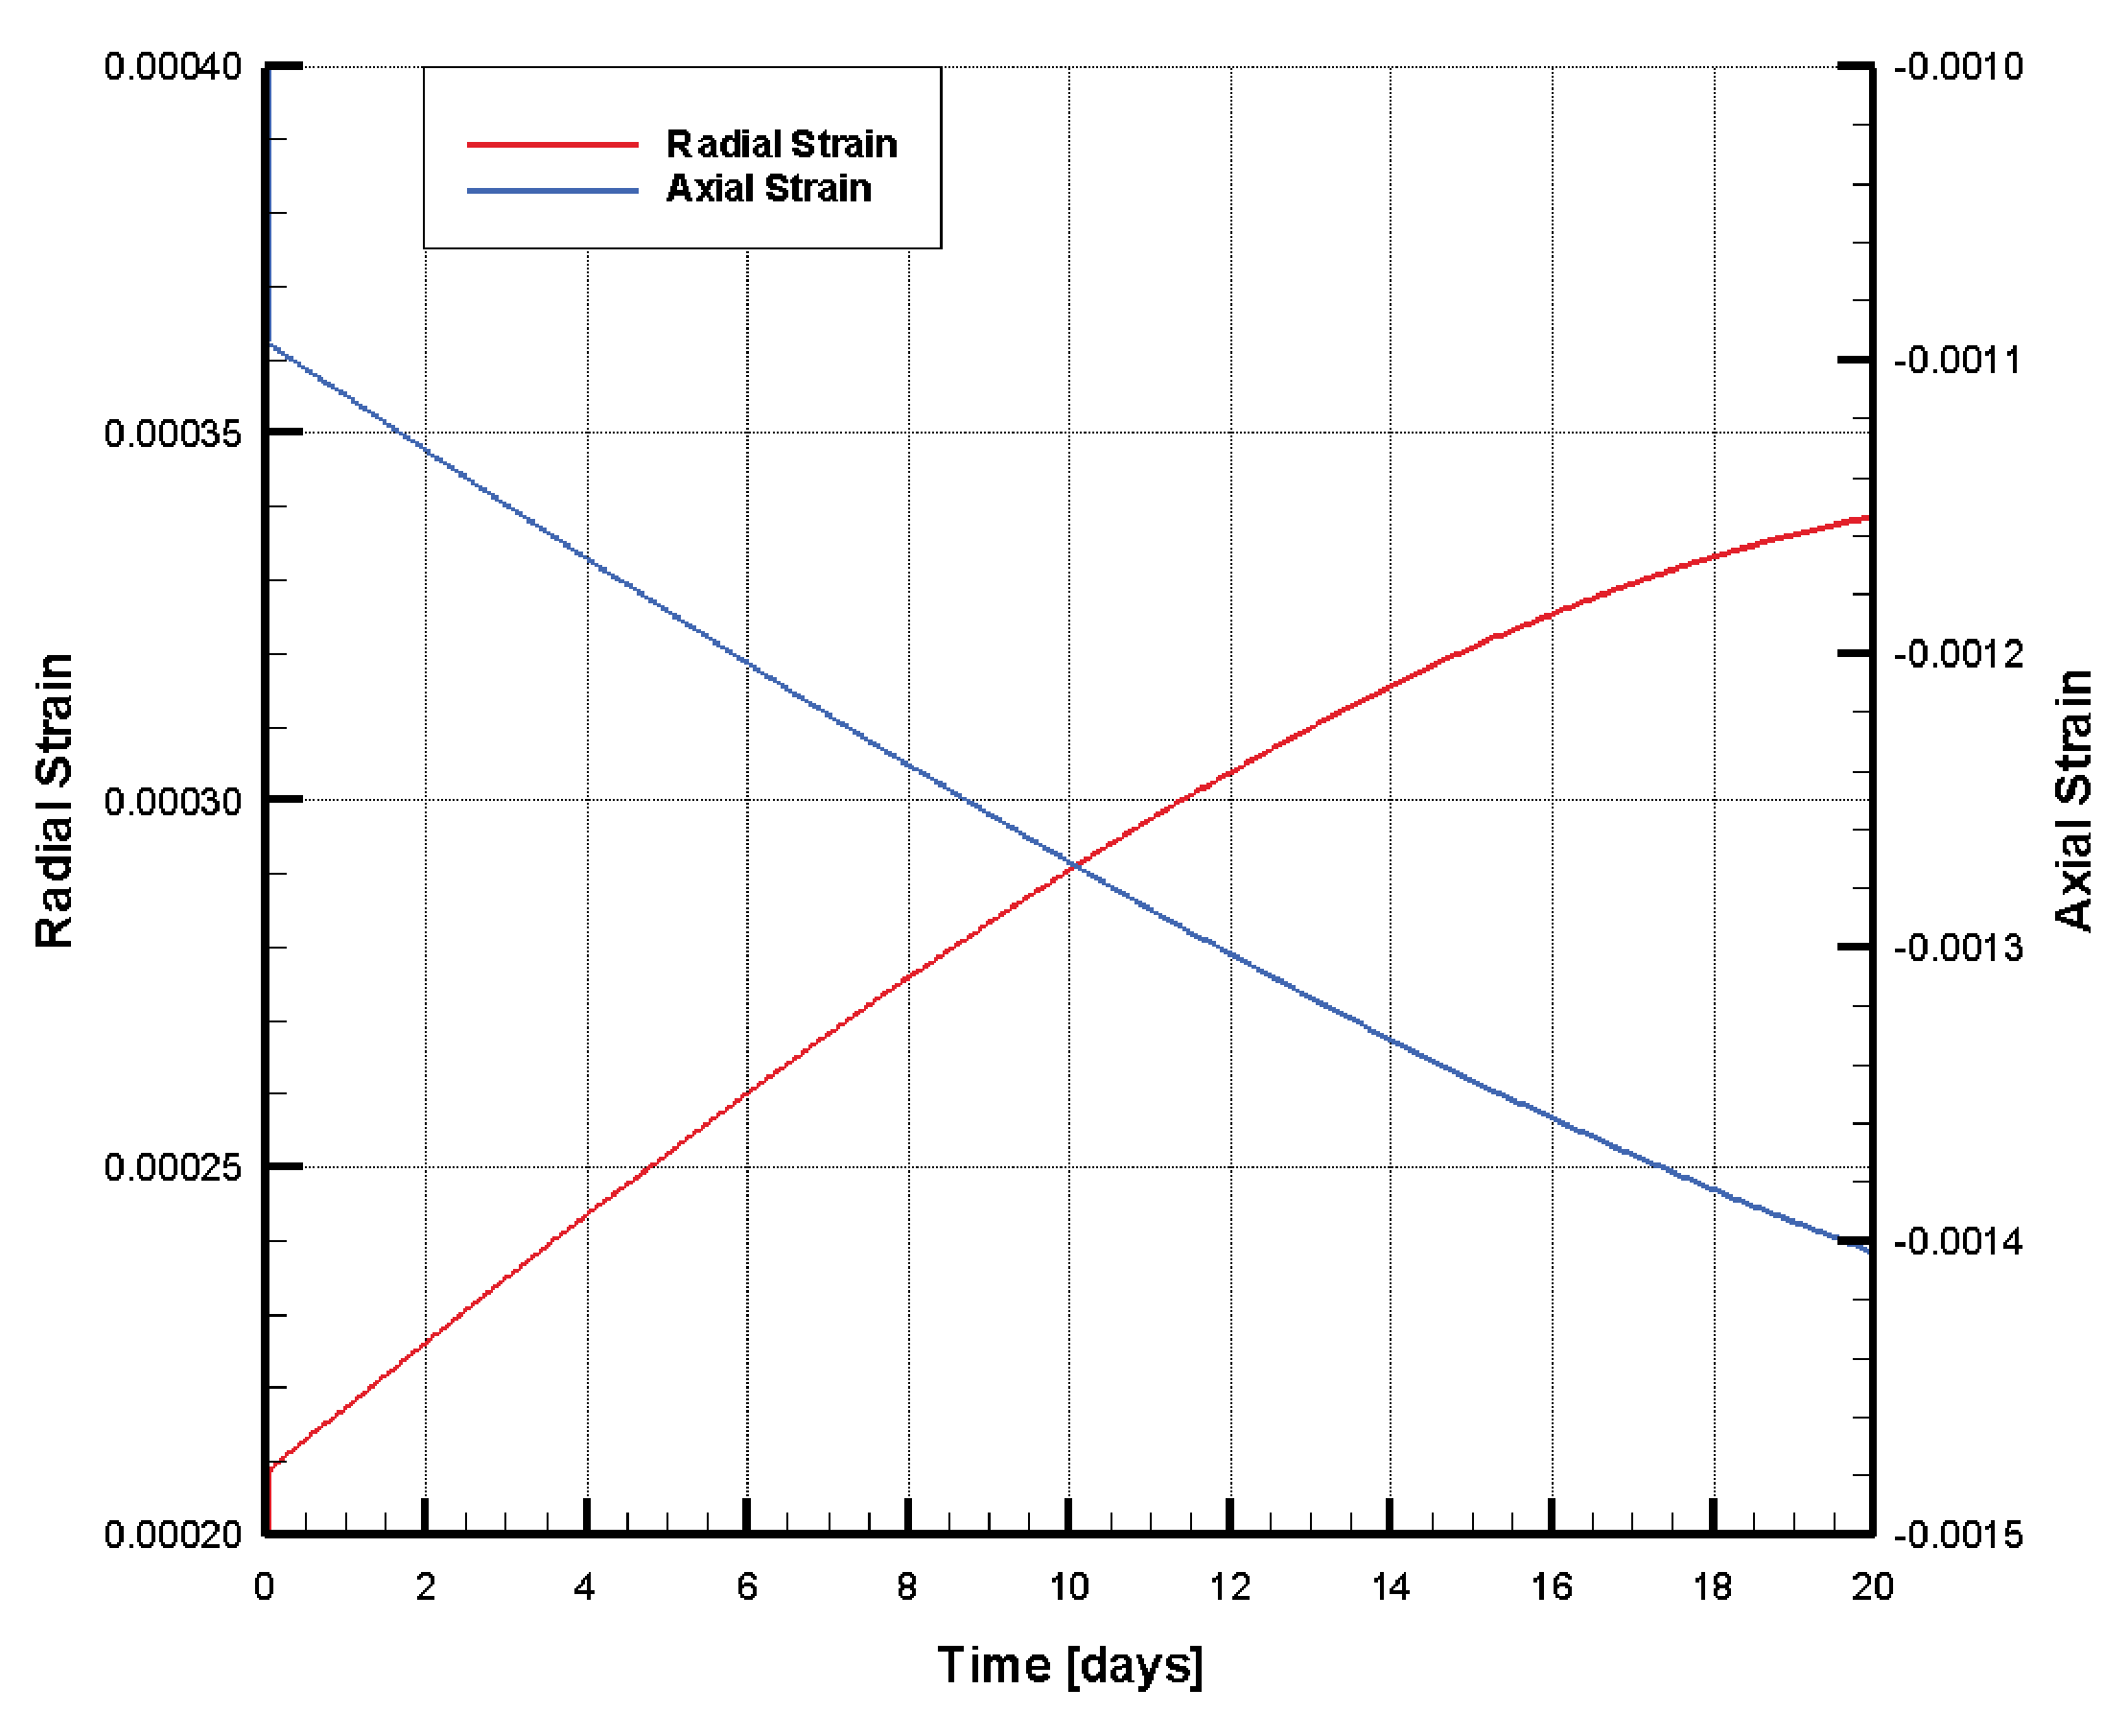
\includegraphics[width=0.6\textwidth]{PART_II/M/svvcreep_e_HL_strain.eps}
\end{center}
\caption{Triaxial compression of a cylindrical sample. Numerical simulation of the transient and stationary creep behavior using the Lubby2 model~(\ref{Mc_lubby2_ec}).} 
\label{Mc_triax_res_lubby2}
\end{figure}
